\documentclass{article}
\title{Notes for: Attention Is All You Need}
\author{Michael N.\thanks{paper: https://arxiv.org/abs/1706.03762}}
\date{\today}
\usepackage{graphicx}


\begin{document}
    \maketitle
    
    \section{High Level and Motivation}
    
    \paragraph{Firstly} As the name suggests, the paper deals with "transformation" tasks such as, among other things, language models (think gpt-2) and machine translation.

    \subsection{Limitations of previous methods}
    \paragraph{RNNs, LSTMs and GRUs} suffer because they are not parallelizable, struggle when they need to maintain long-distance relationships and some of their use-cases in seq-to-seq could be seen as \emph{immoral} (*gasp!*). Are there better solutions?

    \subsubsection{Parallelizable}
    \paragraph{Recurrent models} tend to operate by taking the history of previously generated tokens and predicting the next one conditioned on that history:
    $$p(t_n|t_{n-1}, t_{n-2}, \cdots, t_1, t_0)$$

    \paragraph{} By this definition we can see that if you want to predict 100 tokens, e.g. 100 words, you'll have to follow this sequential process: 
    \begin{enumerate}
        \item predict the first token
        \item predict the next conditioned on the first
        \item predict the next conditioned on the previous two
        \item etc x100.
    \end{enumerate}

    \paragraph{If you wanted to generate} a massive $n$ tokens it will take you $O(n)$ time, and there's no way to parallelize this operation.

    \subsubsection{Long distance relationships}
    
    \paragraph{The vanishing gradient problem} is the problem with RNNs and to a lesser extent LSTMs and GRUs that inputs from many time-steps ago become "diluted" and "lost" amongst newer inputs.
    \paragraph{} This is a concerning issue with NLP and many seq-to-seq tasks in general because, using language as an example, contextual information such as the conversation topic may only be mentioned once at an early time in a sentence. For example, consider this current document, an RNN would have a hard time storing the information that the current topic is the "Limitations of previous methods" because it happened very early on.

    \paragraph{Recurrent Neural Netork}

    $$h_t = f_\theta(h_{t-1}, x_t)$$
    $$h_t = f_\theta(f_\theta(h_{t-2}, x_{t-1}), x_t)$$
    
        As $x_t$, $x_{t-1}$, $\cdots$ are combined, it's likely that unless $\theta$ is configured perfectly there will be a larger likelyhood of $t_0$'s information being "lost".

    \subsubsection{Immorality}

    \paragraph{Is position that important?} RNNs, LSTMs, GRUs and even non-recurrent methods such as Wavenet (which uses CNNs) all capture the spacial relationships of tokens well. However, in problems such as NLP, they don't capture the highly interconnectedness of words. Take for example Winograd schemas...

    \paragraph{Winograd Schema Challenge} Winograd Schema questions simply require the machine to identify the antecedent of an ambiguous pronoun in a statement. 

    \begin{itemize}
        \item The animal didn't cross the street because \emph{it} was too tired.
        \item The animal didn't cross the street because \emph{it} was too wide.
    \end{itemize}

    What is \emph{it}?
    All of the discussed techniques discussed so far fail pitifully (or are not great) at these tasks

    \paragraph{What's needed?} Perhaps some mechanism which relates tokens between each other directly...

    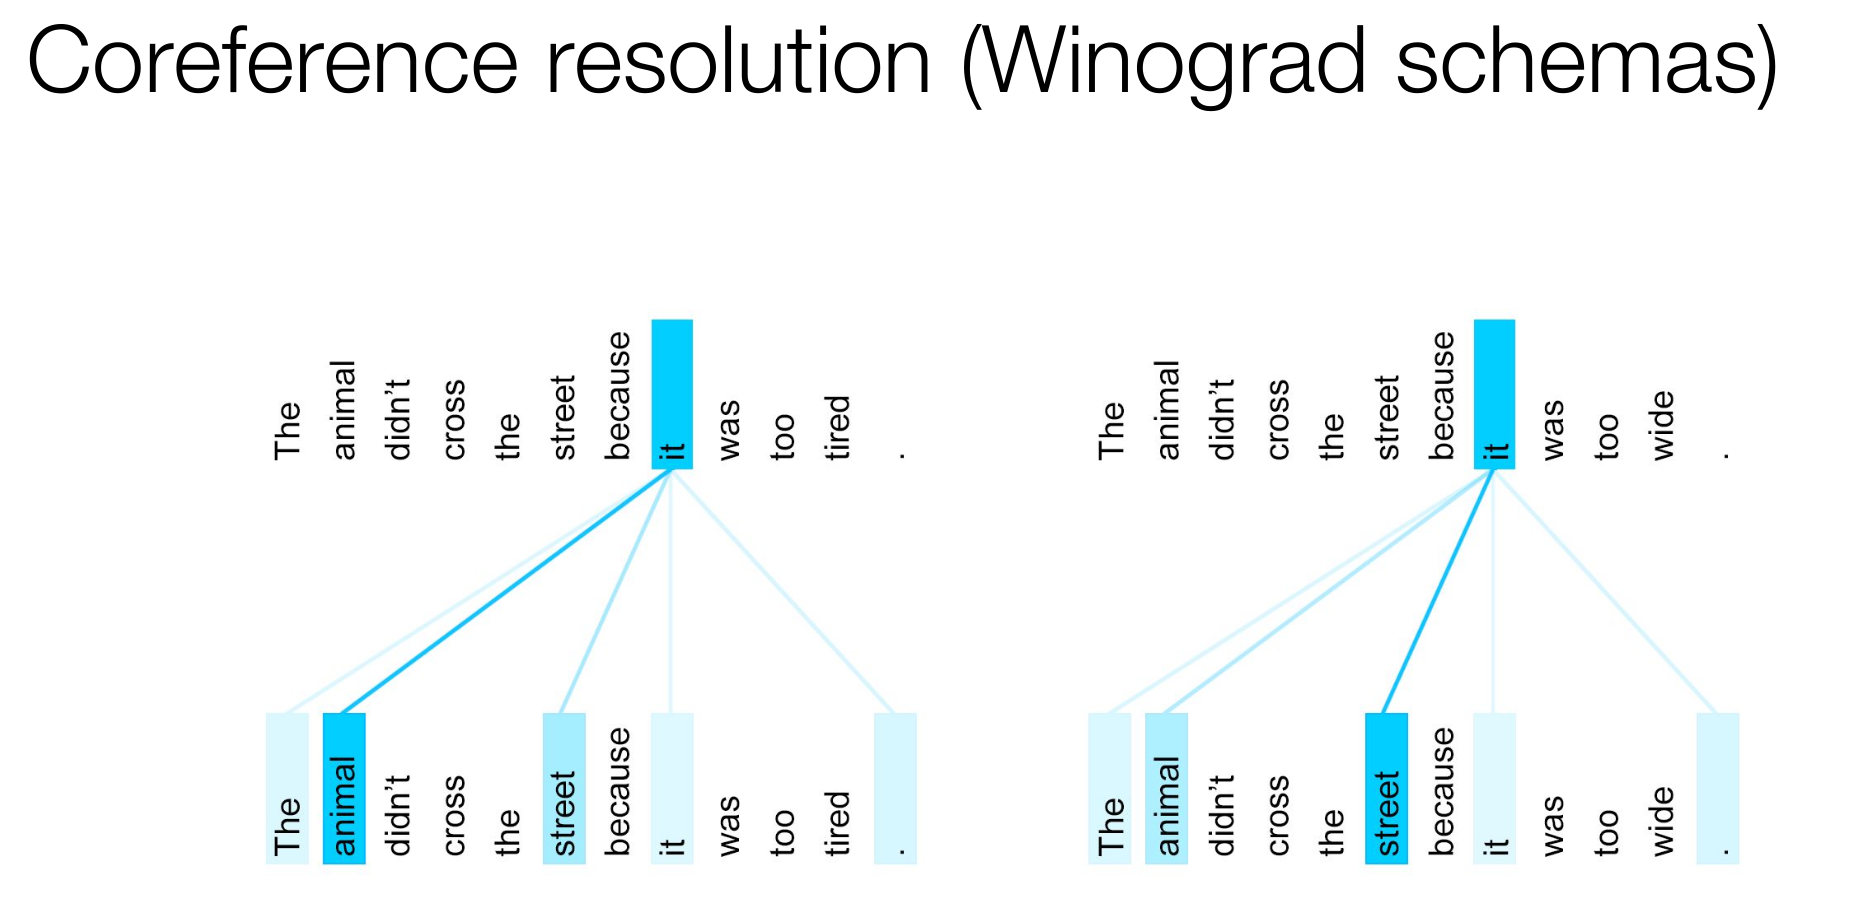
\includegraphics[angle=-90,origin=c,scale=0.1]{fig1.png}

    \section{Core content}



    \section{Their Experiments and Comments}

\end{document}